\documentclass{beamer}
\usepackage{tikz}
\usepackage[utf8]{inputenc}
\usepackage{beamerthemesplit}
\usepackage[english]{babel}
\usepackage{rotating}
\usepackage{amsmath,amsfonts,amssymb,amsthm}
\usepackage{latexsym}
\usepackage{enumerate}
\usepackage{grffile}
\usepackage{listings}
\usepackage{rotating}
\usepackage{color}
\usepackage{wasysym}
\usepackage{algorithm2e}
\usepackage{marvosym}
\usepackage{minted}
\usepackage{multicol}
\usepackage{tipa}
\usepackage{ifsym}
\usepackage{fontawesome}
\usetikzlibrary{calc,shapes.callouts,shapes.arrows,decorations.pathmorphing}

\title{Encrypting Ansible secrets with SOPS}
\author{Felix Fontein}
\date{September 12th, 2023}

\usetheme{Frankfurt}
\setbeamertemplate{navigation symbols}{}

%\setbeamertemplate{background canvas}[vertical shading][bottom=red!10,top=blue!10]
%\usetheme{Warsaw}
%\usefonttheme[onlysmall]{structurebold}

%\newtheorem{definition}{Definition}[section]
%\newtheorem{theorem}[definition]{Theorem}
%\newtheorem{proposition}[definition]{Proposition}
%\newtheorem{lemma}[definition]{Lemma}
%\newtheorem{corollary}[definition]{Corollary}
%\newtheorem{remark}[definition]{Remark}
%\newtheorem{remarks}[definition]{Remarks}
%\newtheorem{example}[definition]{Example}
%\newtheorem{examples}[definition]{Examples}

\newcommand{\N}{\mathbb{N}}
\newcommand{\Z}{\mathbb{Z}}
\newcommand{\Q}{\mathbb{Q}}
\newcommand{\R}{\mathbb{R}}
\newcommand{\C}{\mathbb{C}}
\newcommand{\F}{\mathbb{F}}

\newcommand{\abs}[1]{{\left|{#1}\right|}}
\newcommand{\norm}[1]{{\left\|{#1}\right\|}}
\newcommand{\gen}[1]{{\left\langle{#1}\right\rangle}}
\newcommand{\floor}[1]{{\left\lfloor{#1}\right\rfloor}}
\newcommand{\Matrix}[1]{{\left(\begin{matrix} #1 \end{matrix}\right)}}

\newcommand{\AnsibleLogo}{\raisebox{-1ex}{
\includegraphics[width=3ex]{ansible.pdf}}}

\DeclareFontShape{OT1}{cmtt}{bx}{n}{<5><6><7><8><9><10><10.95><12><14.4><17.28><20.74><24.88>cmttb10}{}

\setbeamerfont{itemize/enumerate body}{size=\Large}
\setbeamerfont{itemize/enumerate subbody}{size=\Large}
\setbeamerfont{itemize/enumerate subsubbody}{size=\footnotesize}

\definecolor{darkgreen}{rgb}{0,0.6,0}
\definecolor{darkred}{rgb}{0.6,0,0}
\definecolor{darkblue}{rgb}{0,0,0.6}
\definecolor{darkyellow}{rgb}{0.6,0.6,0}
\definecolor{lightred}{rgb}{1,0.5,0.5}
\definecolor{lightgreen}{rgb}{0.5,1,0.5}
\definecolor{lightblue}{rgb}{0.5,0.5,1}
\definecolor{lightyellow}{rgb}{1,1,0.5}
\definecolor{lightgray}{gray}{0.75}
\definecolor{verylightgray}{gray}{0.95}

\newcount\fadein
\newcount\fadeout
\newcount\colorfade
\newdimen\shift

\definecolor{mygreen}{rgb}{0,0.6,0}
\definecolor{mygray}{rgb}{0.5,0.5,0.5}
\definecolor{mymauve}{rgb}{0.58,0,0.82}
\lstset{language=python,
        basicstyle=\large\tt,
        commentstyle=\color{mygreen},
        keywordstyle=\color{blue},
        stringstyle=\color{mymauve},
        numbers=left,
        numberstyle=\tiny\color{mygray},
        stepnumber=1,
        numbersep=5pt}

\makeatletter
\newlength\beamerleftmargin
\setlength\beamerleftmargin{\Gm@lmargin}
\makeatother

\begin{document}

  \frame{\titlepage}

  \begin{frame}
    \frametitle{Roadmap}
    \tableofcontents%[pausesections]
  \end{frame}

  \section{Unrelated things}
  \begin{frame}
    \frametitle{Who am I?}
    
    \begin{block}{Felix Fontein (\textipa{"fe:lIks "fOnta\textsubarch{I}n})}
      \begin{tabular}{lll}
        \Letter\ \href{mailto:felix@fontein.de}{felix@fontein.de}
        &
        \qquad
        \qquad
        &
        felixfontein (Libera.Chat)
        \\
        \faGithub\ \href{https://github.com/felixfontein/}{@felixfontein}
        &
        \qquad
        \qquad
        &
        felixfontein:matrix.org (Matrix)
      \end{tabular}
    \end{block}
    
    \begin{block}{Ansible contributor}
      \begin{itemize}
        \item \normalsize (co-)maintainer of several community collections
          \begin{itemize}
            \item[$\rightarrow$] \normalsize among them community.sops
          \end{itemize}
        \item co-maintainer of antsibull tools
        \item member of \href{https://docs.ansible.com/ansible/devel/community/steering/steering_index.html}{Ansible Community Steering Committee}
      \end{itemize}
    \end{block}
    
    \begin{block}{SOPS contributor}
      co-maintainer of SOPS (for 3 weeks by now)
    \end{block}
  \end{frame}

  \begin{frame}
    \frametitle{Ansible Forum}
    \vspace{-0.25cm}
    \begin{center}
      Officially available since September 11th:
      
      \vspace{0.2cm}
      
      \alert{\Huge \href{https://forum.ansible.com}{forum.ansible.com}}
      
      \vspace{0.1cm}
    \end{center}

    \hspace*{-\beamerleftmargin}%
    \href{https://forum.ansible.com}{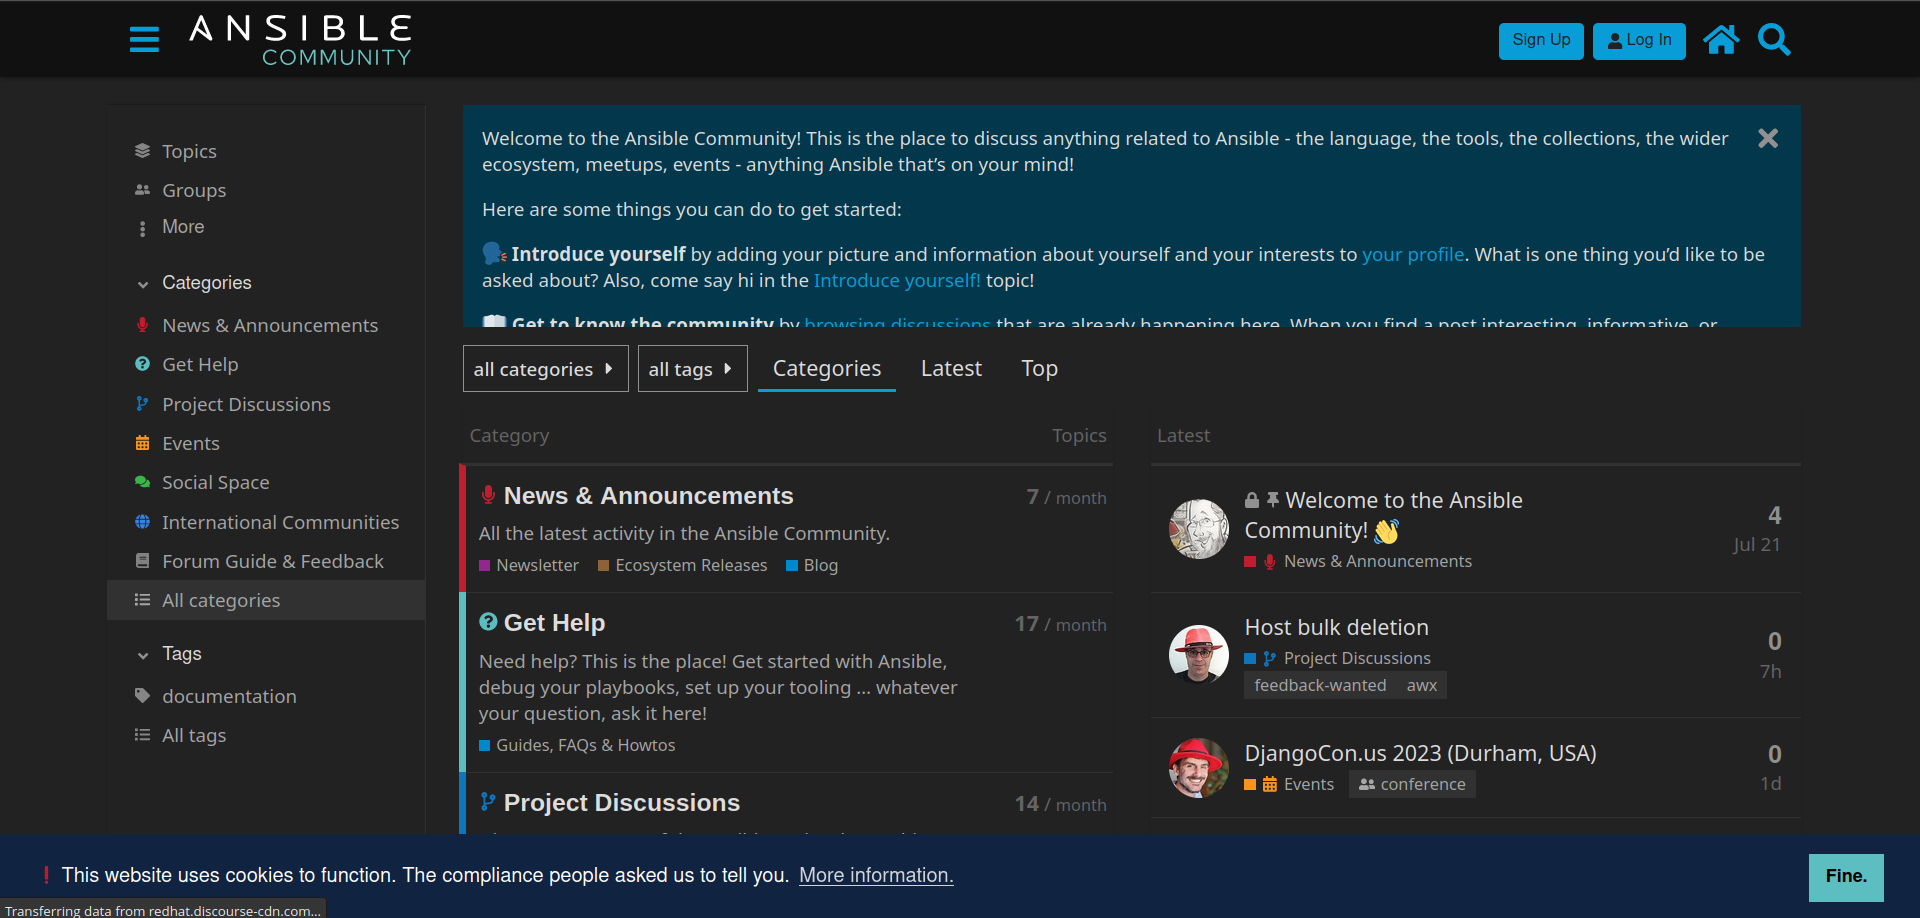
\includegraphics[width=\paperwidth]{../source/ansible-forum.png}}
  \end{frame}

  \section{What is SOPS?}
  \begin{frame}
    \frametitle{SOPS: Secrets OPerationS (1/3)}
    \begin{itemize}
      \item \alert{Secret handling tool} \url{https://github.com/getsops/sops}
      \item<2-> Handles \alert{structured data:} YAML, JSON, INI, ...
      \begin{itemize}
        \item ... but also binary files (Base64);
        \item keys are not encrypted;
        \item values and comments are encrypted.
      \end{itemize}
      \item<3-> \alert{Multiple identities} can have access
      \begin{itemize}
        \item GPG, Age, AWS KMS, Google Cloud KMS, Azure Key Vault, Hashicorp Vault
        \item supports \textbf{Shamir's Secret Sharing} (need access to multiple identities to decrypt)
      \end{itemize}
    \end{itemize}
  \end{frame}

  \begin{frame}
    \frametitle{SOPS: Secrets OPerationS (2/3)}
    \begin{itemize}
      \item Written and originally maintained by (ex-)Mozilla employees
      \item Effectively unmaintained since June 2022
      \begin{itemize}
        \item A lot of community PRs, but no way to get them merged...
        \item Or get a new release with some already merged bugfixes out...
      \end{itemize}
      \item<2-> February 2023: SOPS has applied to be adopted into the CNCF sandbox
      \item<2-> May 2023: \alert{CNCF sandbox application accepted!}
      \item<3-> August 25th: 3.8.0-rc.1 pre-release
    \end{itemize}
  \end{frame}

  \begin{frame}[fragile]
    \frametitle{SOPS: Secrets OPerationS (3/3)}
    \begin{itemize}
      \item Quick demo!
      \item Contents:
        \begin{itemize}
          \item \lstinline{.sops.yaml} config
          \item \lstinline{example.sops.yaml} file
        \end{itemize}
    \end{itemize}
  \end{frame}

  \section{How does it compare to Ansible Vault?}
  \begin{frame}
    \frametitle{SOPS vs. Ansible Vault}
    \vspace{-0.75cm}
    \begin{columns}[t]
      \begin{column}{0.5\textwidth}
        \begin{block}{SOPS}
          \begin{itemize}
            \item[\color{blue}$\odot$] asymmetric crypto
            \item[\color{darkgreen}$\oplus$]<2-> multiple identities per file
            \item[\color{darkgreen}$\oplus$]<3-> no service needed
            \item[\color{darkred}$\ominus$]<4-> no native \AnsibleLogo\ support
          \end{itemize}
        \end{block}
        \vspace{1cm}
        \begin{flushright}
          \begin{minipage}{0.8\textwidth}
            \begin{flushright}
              HashiVault, BitWarden, OnePasword, ...
            \end{flushright}
          \end{minipage} $\longrightarrow$
        \end{flushright}
      \end{column}
      \begin{column}{0.5\textwidth}
        \begin{block}{Ansible Vault}
          \begin{itemize}
            \item[\color{blue}$\odot$] symmetric crypto
            \item[\color{darkred}$\ominus$]<2-> one passphrase per file
            \item[\color{darkgreen}$\oplus$]<3-> no service needed
            \item[\color{darkgreen}$\oplus$]<4-> native \AnsibleLogo\ support
          \end{itemize}
        \end{block}
        \vspace{-0.15cm}
        \begin{block}{Other service (via plugin)}
          \begin{itemize}
            \item[\color{blue}$\odot$] "trust by contract"
            \item[\color{darkgreen}$\oplus$]<2-> access management
            \item[\color{darkred}$\ominus$]<3-> needs service
            \item[\color{darkred}$\ominus$]<4-> no native \AnsibleLogo\ support
          \end{itemize}
        \end{block}
      \end{column}
    \end{columns}
  \end{frame}

  \section{Using SOPS with community.sops}
  \begin{frame}
    \frametitle{Ansible community.sops collection}
    
    \begin{itemize}
      \item Originally PR for \lstinline{sops} lookup plugin in ansible/ansible
      \item Merged into community.general after the big collection split
      \item ... and moved to own collection a few days later (June 2020)
    \end{itemize}
  \end{frame}
  
  \begin{frame}
    \frametitle{Ansible community.sops collection: roles and playbooks}
    
    \begin{block}{Roles}
      \begin{itemize}
        \item \lstinline{community.sops.install}
      \end{itemize}
    \end{block}
    
    \begin{block}{Playbooks}
      \begin{itemize}
        \item \lstinline{community.sops.install}
        \item \lstinline{community.sops.install_localhost}
          \begin{itemize}
            \item[$\rightarrow$] Useful for setting up Execution Environments
          \end{itemize}
      \end{itemize}
    \end{block}
  \end{frame}
  
  \begin{frame}[fragile,t]
    \frametitle{Ansible community.sops collection: plugins}
    \begin{itemize}
      \item \href{https://docs.ansible.com/ansible/devel/collections/community/sops/}{Documentation on docs.ansible.com}
      \item \alert<2>{Vars plugin: \lstinline{community.sops.sops}}
      \item \alert<3>{Action plugin: \lstinline{community.sops.load_vars}}
      \item \alert<4>{Lookup: \lstinline{community.sops.sops}}
      \item \alert<5>{Filter: \lstinline{community.sops.decrypt}}
      \item \alert<6>{Module: \lstinline{community.sops.sops_encrypt}}
    \end{itemize}
    \only<2>{\begin{block}{Vars plugin \lstinline{community.sops.sops}}
      Load encrypted files directly from \lstinline{host_vars} and \lstinline{group_vars} as \AnsibleLogo variables.
    \end{block}}
    \only<3>{\begin{block}{Action plugin \lstinline{community.sops.load_vars}}
      Load encrypted file similar to \lstinline{ansible.builtin.include_vars} as \AnsibleLogo facts. \\
      \alert{Caveat:} interpolation must be done at load time.
    \end{block}}
    \only<4>{\begin{block}{Lookup \lstinline{community.sops.sops}}
      Load encrypted file from disk:
      \lstinline{lookup('community.sops.sops', '/path/to/file')}.
    \end{block}}
    \only<5>{\begin{block}{Filter \lstinline{community.sops.decrypt}}
      Decrypt data in Jinja2 expressions:
      \lstinline{encrypted_data | community.sops.decrypt}.
    \end{block}}
    \only<6>{\begin{block}{Module \lstinline{community.sops.sops_encrypt}}
      Encrypt data with SOPS, for example output of another task:
      \lstinline{community.crypto.openssl_privatekey_pipe} → \lstinline{community.sops.sops_encrypt}
    \end{block}}
  \end{frame}

  \begin{frame}[fragile,t]
    \frametitle{Load encrypted data files as variables}
    \begin{minted}[gobble=6, frame=single, linenos]{yaml}
      - hosts: webserver
        vars_files:
          - data/letsencrypt.yml
        pre_tasks:
          - name: Load encrypted credentials
            community.sops.load_vars:
              file: keys/credentials.sops.yml
              expressions: ignore  # or: evaluate-on-load
            tags: always
            no_log: true
        roles:
          - ...
    \end{minted}
    \begin{block}{Note}
      Expressions must be evaluated on load time ($\neq$ \lstinline{include_vars}).
    \end{block}
  \end{frame}

  \begin{frame}[fragile,t]
    \frametitle{Create or update SOPS encrypted private key}
    \vspace{-2ex}
    \begin{minted}[gobble=6, frame=single, linenos]{yaml+jinja}
      - block:
       - community.crypto.openssl_privatekey_pipe:
          content: "{{lookup('community.sops.sops',
           'keys/private_key.pem.sops',
           empty_on_not_exist=true)|default(omit,true)}}"
         no_log: true
         register: private_key_temp

       - community.sops.sops_encrypt:
          path: keys/private_key.pem.sops
          content_text: "{{private_key_temp.privatekey}}"
         when: private_key_temp.changed

       always:
       - ansible.builtin.set_fact:
          private_key_temp: ''
    \end{minted}
  \end{frame}

  \begin{frame}[fragile]
    \frametitle{More demos!}
    \begin{itemize}
      \item Demo!
    \end{itemize}
  \end{frame}

  \section*{}
  \begin{frame}
    \begin{center}
      \Huge Thank You\\
      for your attention!

      \vspace{1.5cm}

      \LARGE Questions? Comments?
      
      \vspace{1.5cm}
      
      \small \href{https://github.com/felixfontein/ansible-meetup-20230912-zurich-demo}{Link to demo repository}
    \end{center}
  \end{frame}
\end{document}
